\iffalse
\let\negmedspace\undefined
\let\negthickspace\undefined
\documentclass[journal,12pt,twocolumn]{IEEEtran}
\usepackage{cite}
\usepackage{amsmath,amssymb,amsfonts,amsthm}
\usepackage{algorithmic}
\usepackage{graphicx}
\usepackage{textcomp}
\usepackage{xcolor}
\usepackage{txfonts}
\usepackage{listings}
\usepackage{enumitem}
\usepackage{mathtools}
\usepackage{gensymb}
\usepackage{comment}
\usepackage[breaklinks=true]{hyperref}
\usepackage{tkz-euclide} 
\usepackage{listings}
\usepackage{gvv}                                        
\def\inputGnumericTable{}                                 
\usepackage[latin1]{inputenc}                                
\usepackage{color}                                            
\usepackage{array}                                            
\usepackage{longtable}                                       
\usepackage{calc}                                             
\usepackage{multirow}                                         
\usepackage{hhline}                                           
\usepackage{ifthen}                                           
\usepackage{lscape}
\usepackage{caption}
\newtheorem{theorem}{Theorem}[section]
\newtheorem{problem}{Problem}
\newtheorem{proposition}{Proposition}[section]
\newtheorem{lemma}{Lemma}[section]
\newtheorem{corollary}[theorem]{Corollary}
\newtheorem{example}{Example}[section]
\newtheorem{definition}[problem]{Definition}
\newcommand{\BEQA}{\begin{eqnarray}}
\newcommand{\EEQA}{\end{eqnarray}}
\newcommand{\define}{\stackrel{\triangle}{=}}
\theoremstyle{remark}
\newtheorem{rem}{Remark}
\begin{document}

\bibliographystyle{IEEEtran}
\vspace{3cm}

\title{10.5.2.14}
\author{EE23BTECH11003 - pranav}
\maketitle
\newpage

\bigskip
\renewcommand{\thefigure}{\arabic{figure}}
\renewcommand{\thetable}{\arabic{table}}

\textbf{Question}:Given that $\frac{dy}{dx}=2x+y$ and $y=1$,when $x=0$ Using Runge-Kutta fourth order method,the value of $y$ at $x=0.2$ is \hfill(GATE 2023 AG 50) 
\solution
\fi
By using runge kutta 4 th order method\\
\begin{table}[h]
    \centering
    \input{2023/AG/50/tables/Table.Tex}
    \caption{Variables Used}
\end{table}
\begin{align}
y(n)=y(n-1)+\frac{h}{6}[(2x(n-1)+y(n-1)(6+3h+h^2+\frac{h^3}{4})+(6h+2h^2+\frac{h^3}{2})]
\end{align}
assume step size as $0.1$ and initial conditions as $x=0$ and $y=1$\\
\begin{align}
y(n)&=1+(6+3(0.1)+0.1^2+\frac{0.1^3}{4})+(6(0.1)+2(0.1)^2+\frac{0.1^3}{2})\\
\implies y_{n}&=1.115
\end{align}
cosidering outputs of last iteration as inputs of next iteration\\
\begin{align}
y(n)=1.155+\frac{0.1}{6}[(2(0.1)+1.155(6+3(0.1)+(0.1)^2+\frac{(0.1)^3}{4})+(6(0.1)+2(0.1)^2+\frac{(0.1)^3}{2})]
\implies y(n)=1.29
\end{align}
so at $x=0.2$ value of $y$ is $1.29$\\
analysis
\begin{align}
\frac{dy}{dx}&=2x+y\\
ye^{-x}&=\int2xe^{-x}dx\\
\implies ye^{-x}&=-2(x+1)e^{-x}+c
\end{align}
by using intial conditions
\begin{align}
c=3\\
\implies y=3e^x-2(x+1)
\end{align}
\newpage
\begin{figure}
    \centering
    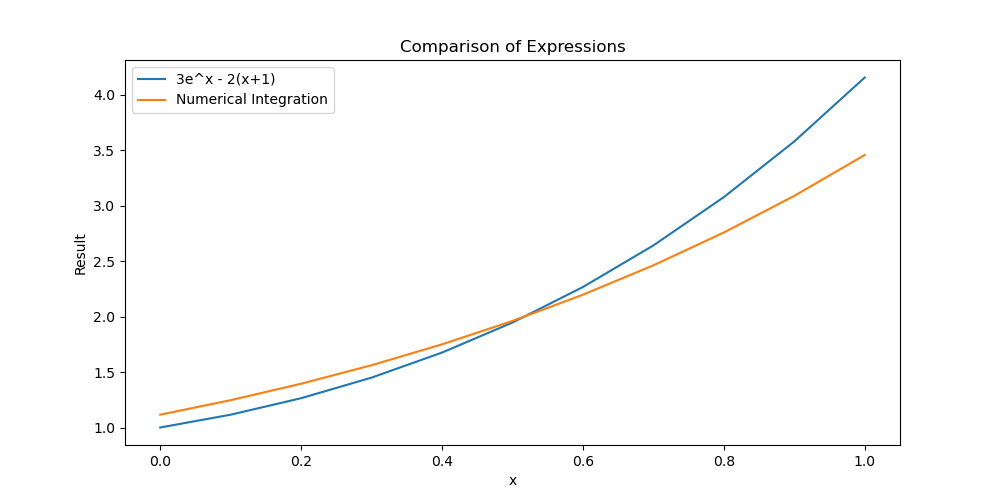
\includegraphics[width=1\linewidth]{2023/AG/50/figs/grap.png}
    \caption{simulation vs analysis}
\end{figure}

%\end{document}
